\section{Diskussion}
\label{sec:Diskussion}
Sinusgenerator nicht gut einstellbar: Bei drehung keine garantie von änderung in diese Richtung
Andere einstellungen als in der Anleitung
keine feine einstellbarkeit des Sinusgenerators
schwierigkeiten das ergebnis am AC-Millivoltmeter abzulesen
teilweise unterschiedliche Ausgangsspannungen bei denselben 
\section{Anhang}
\label{sec:Anhang}
\begin{figure}
    \centering
    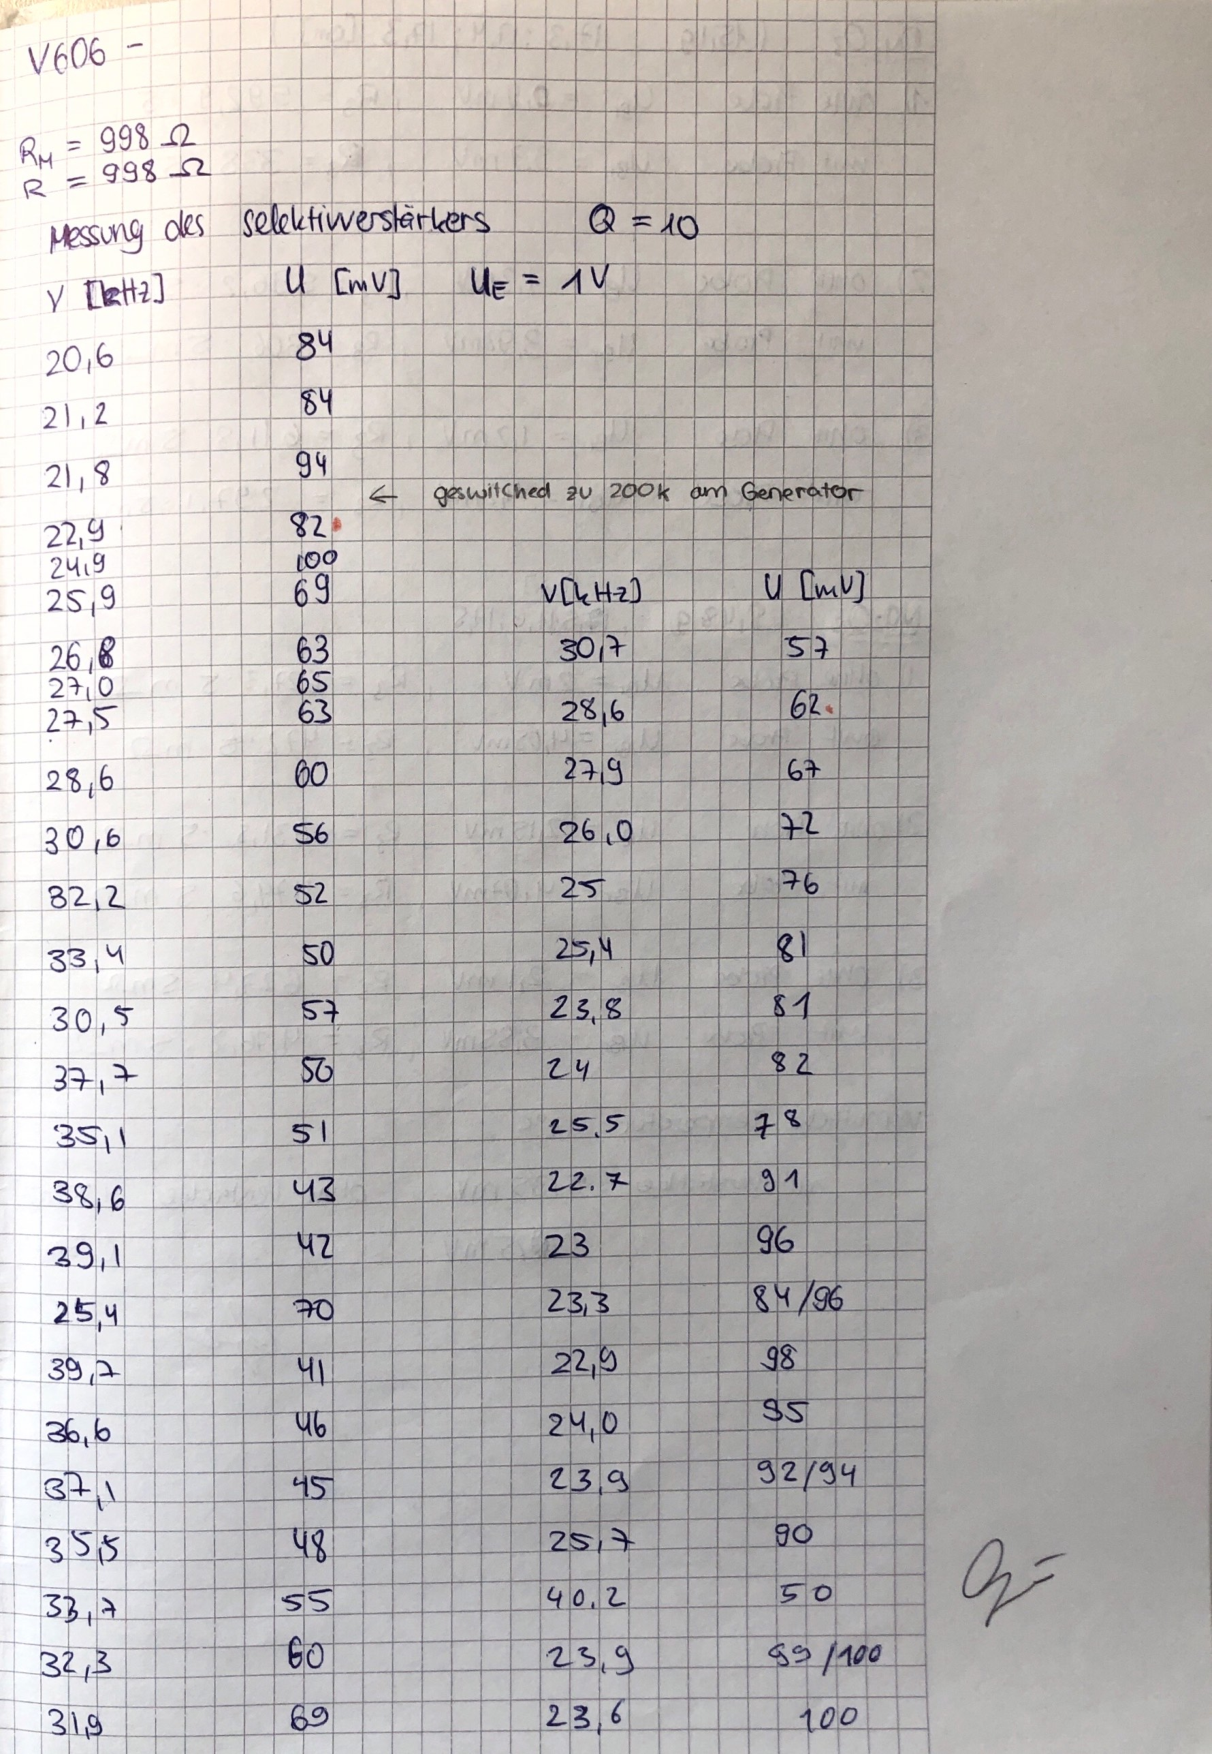
\includegraphics[width=\textwidth]{content/datenselektiv.pdf}
    \caption{Die aufgenommenen Werte für die Messung der Filterkurve des Selektivverstärkers.}
    \label{fig:datenselektiv}
\end{figure}
\begin{figure}
    \centering
    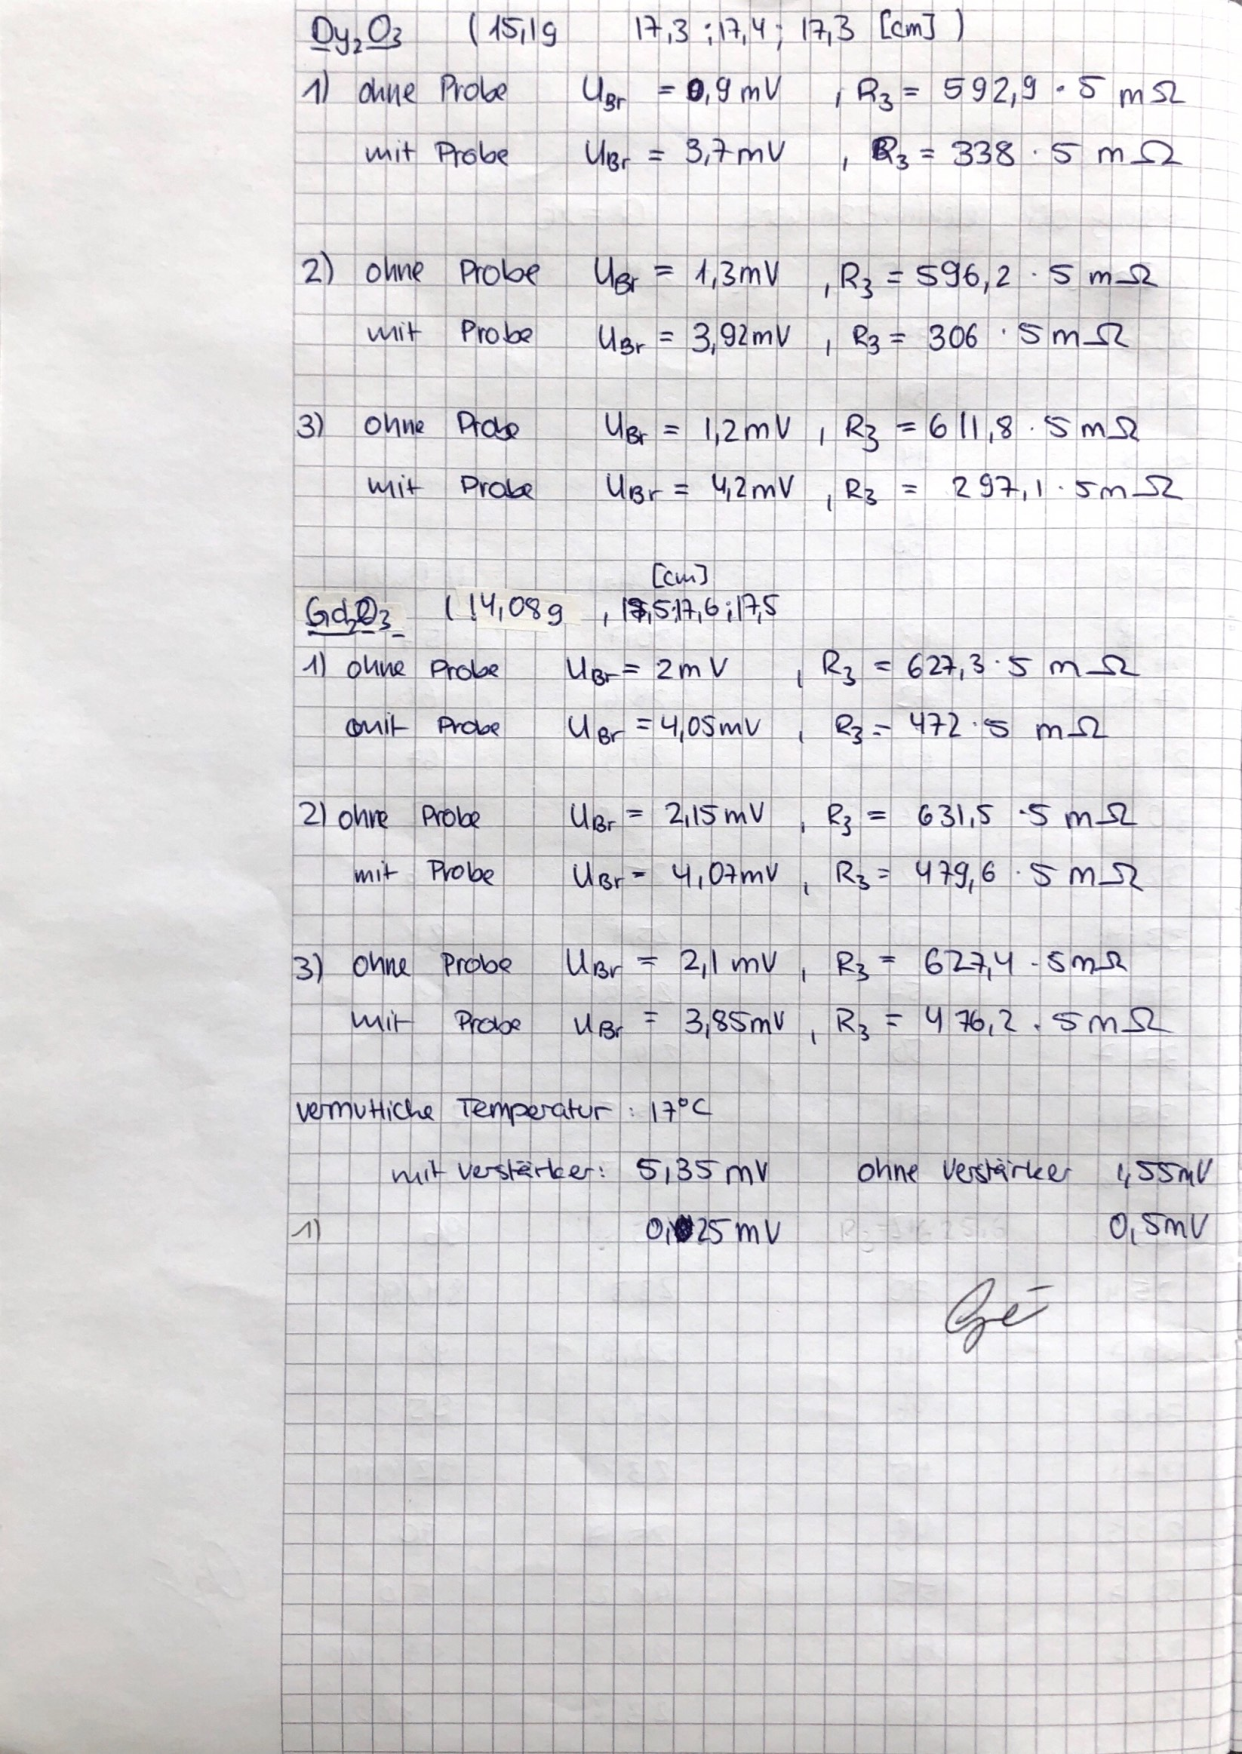
\includegraphics[width=\textwidth]{content/datenmessung.pdf.pdf}
    \caption{Die notierten Werte von der Vermessung der paramagnetischen Proben.}
    \label{fig:datenmessung}
\end{figure}